After implementing the verilog code.
We used the timing function to verify the working of the code.
Below, we are attaching the screenshots from the timing diagram

\subsection{ADD Operation:}\label{subsec:add-operation}
Below figure \ref{fig:timing add} shows the \textbf{ADD} operation between two binary \textit{A = 1111 and B = 1111} numbers
where the result is stored in register \textit{C} sequentially in each clock cycles.
\begin{figure}[H]
    \begin{center}
        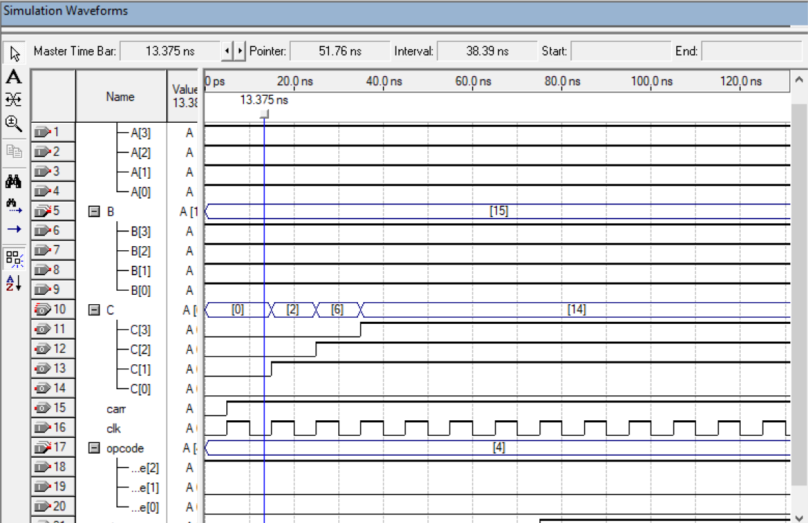
\includegraphics[width = 0.4\textwidth]{figures/add}
    \end{center}
    \caption{Timing Daigram for ADD Operation}
    \label{fig:timing add}
\end{figure}

\subsection{SUB Operation}\label{subsec:sub-operation}
Below figure \ref{fig:timing sub} shows the \textbf{SUB} operation between two binary \textit{A = 0111 and B = 0111} where the output \textit{C} = \textit{0000}.
As we are working with signed number, the numbers are represented as \textbf{2s complement}.

\begin{figure}[H]
    \begin{center}
        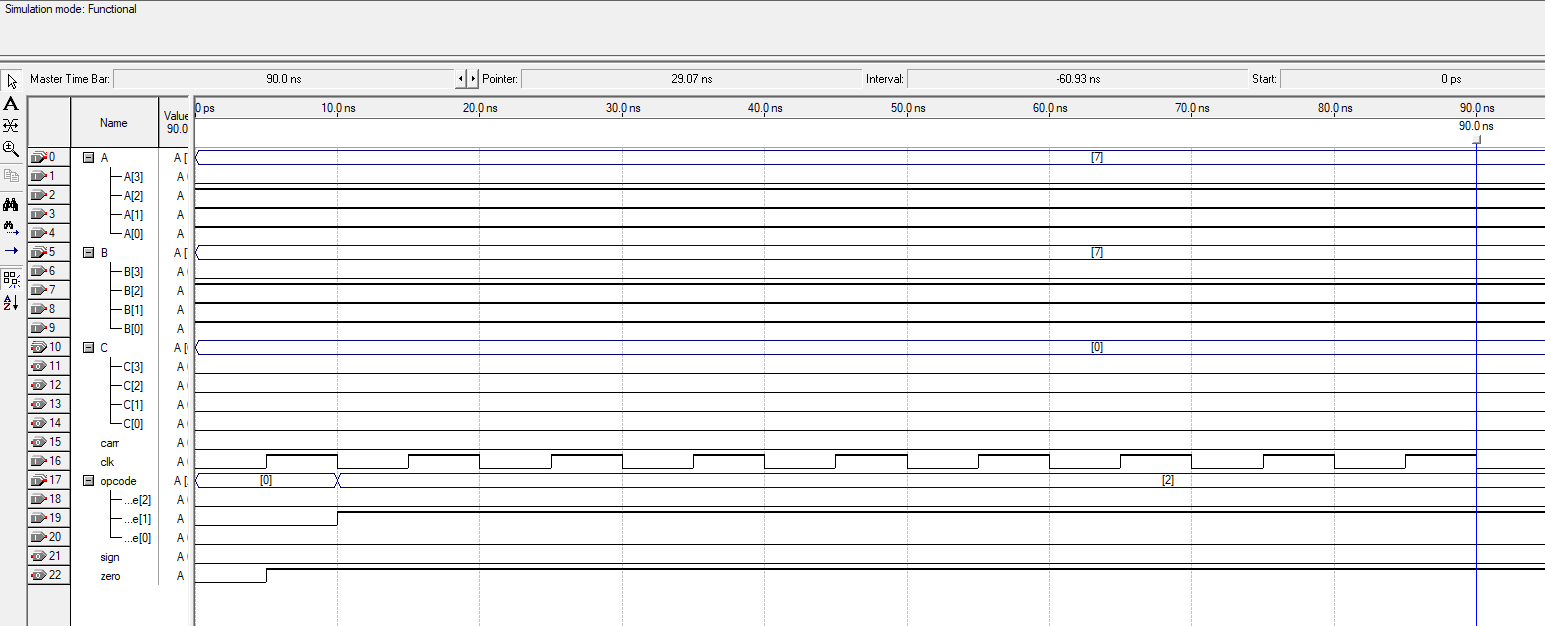
\includegraphics[width = 0.4\textwidth]{figures/Sub_Operation}
    \end{center}
    \caption{Timing Diagram for Sub Operation}
    \label{fig:timing sub}
\end{figure}

\textbf{NAND} and \textbf{XNOR} operation are pretty much straight forward.
All we had to do is put the equation in the verilog and then the
operation performed as expected.
Below timing diagram, those operations are attached.

\subsection{NAND Operation}\label{subsec:nand-operation}

\begin{figure}[H]
    \begin{center}
        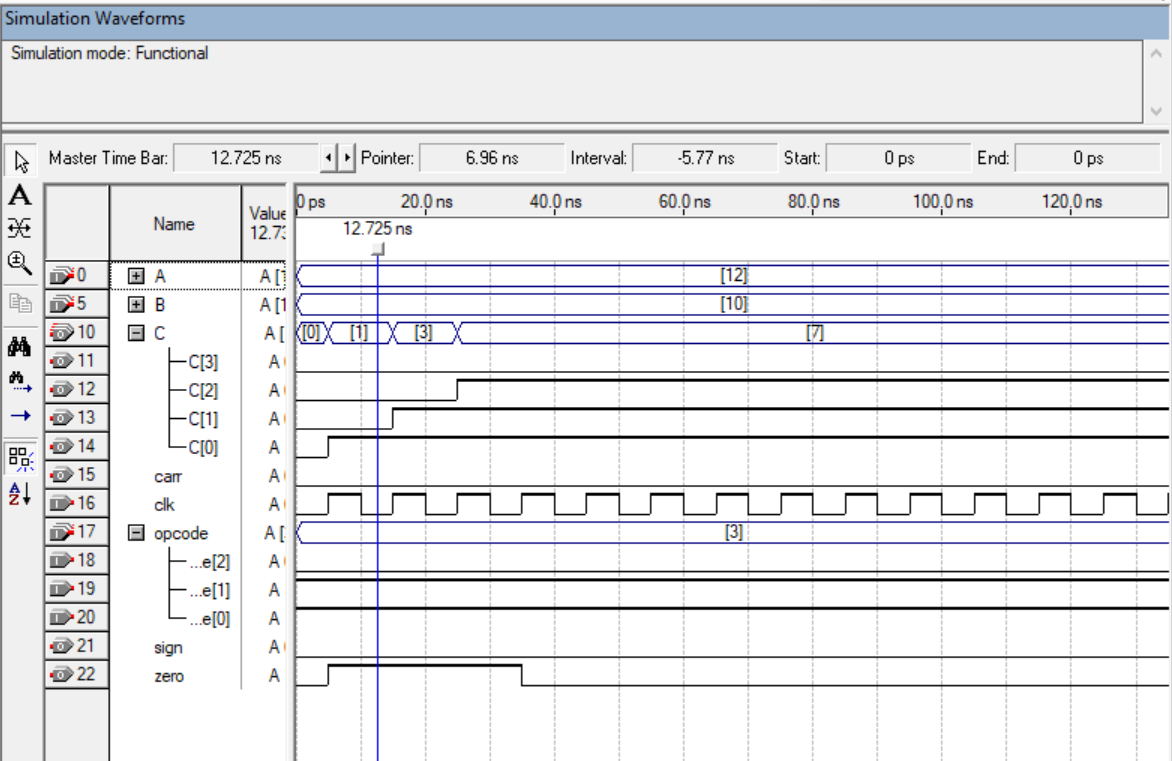
\includegraphics[width = 0.4\textwidth]{figures/nand}
    \end{center}
    \caption{Timing Daigram for NAND Operation}
    \label{fig:timing nand}
\end{figure}

\subsection{XNOR Operation}\label{subsec:xnor-operation}
\begin{figure}[H]
    \begin{center}
        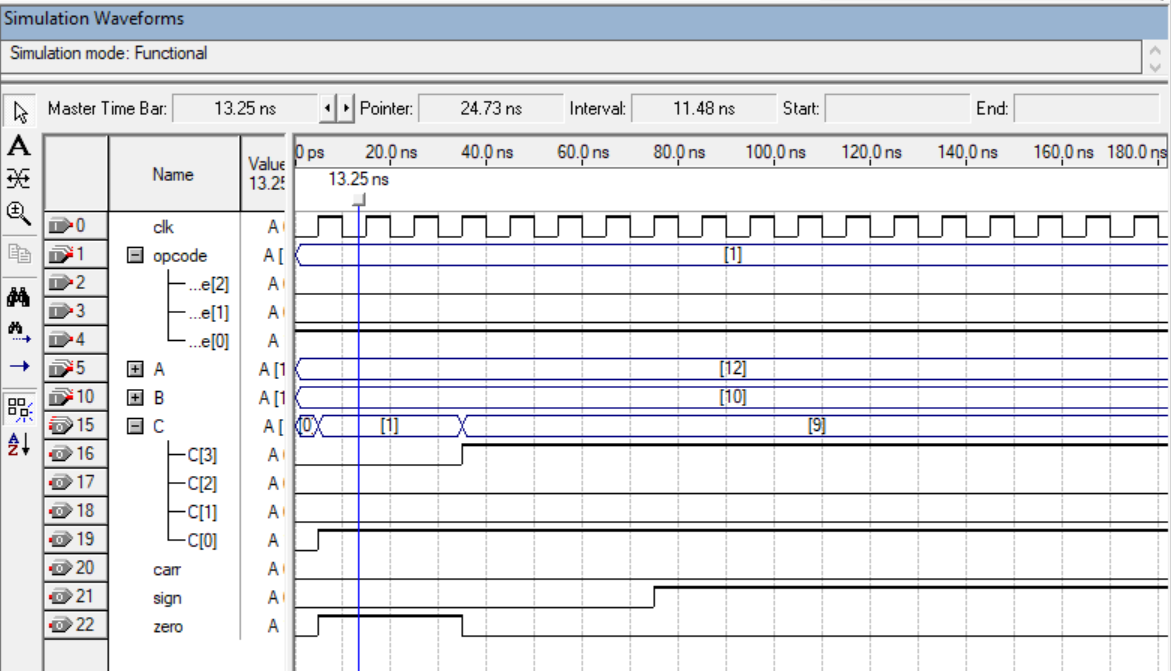
\includegraphics[width = 0.4\textwidth]{figures/xnor}
    \end{center}
    \caption{Timing Daigram for XNOR Operation}
    \label{fig:timing xnor}
\end{figure}

\subsection{Multiple Operation With Reset}\label{subsec:multiple-operation-with-reset}
The below attached Figure \ref{fig:multiple operation} shows multiple Operations with \textbf{SET} and \textbf{RESET} functionality.
At first the \textbf{ADD} operation is performed between binary number \textit{0001} and \textit{0111}.
After that, the \textbf{opcode} is changed to RESET which is \textit{000} during time \textit{50ns} to \textit{60ns}.
Next the \textbf{opcode} was changed to \textit{010} and performed \textbf{SUB} operation during the next \textbf{8} clock cycles or two \textbf{BUS} cycles.
After that the mandatory \textbf{RESET} and then \textbf{NAND} operation for another 4 cycles as the \textit{opcode} was changed to \textit{011}.
\begin{figure}[H]
    \begin{center}
        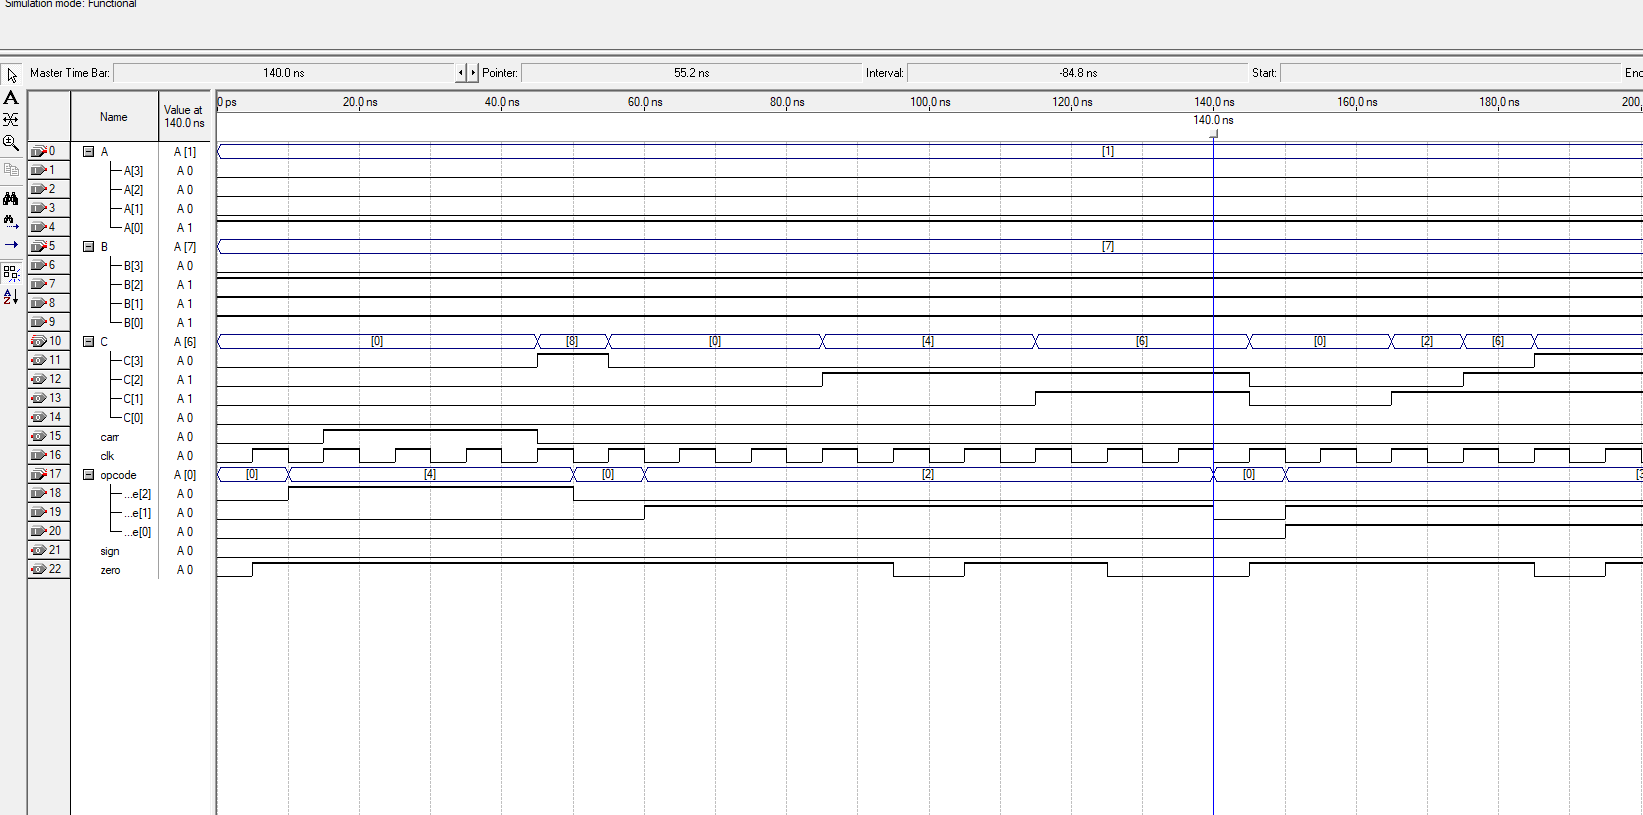
\includegraphics[width = 0.4\textwidth]{figures/Multiple_Operations}
    \end{center}
    \caption{Timing Daigram with reset}
    \label{fig:multiple operation}
\end{figure}
